\chapter{Background}

\section{Automatic Identification Systems (AIS)}

\begin{figure}[htbp]  % order of priority: h here, t top, b bottom, p page
    \centering
    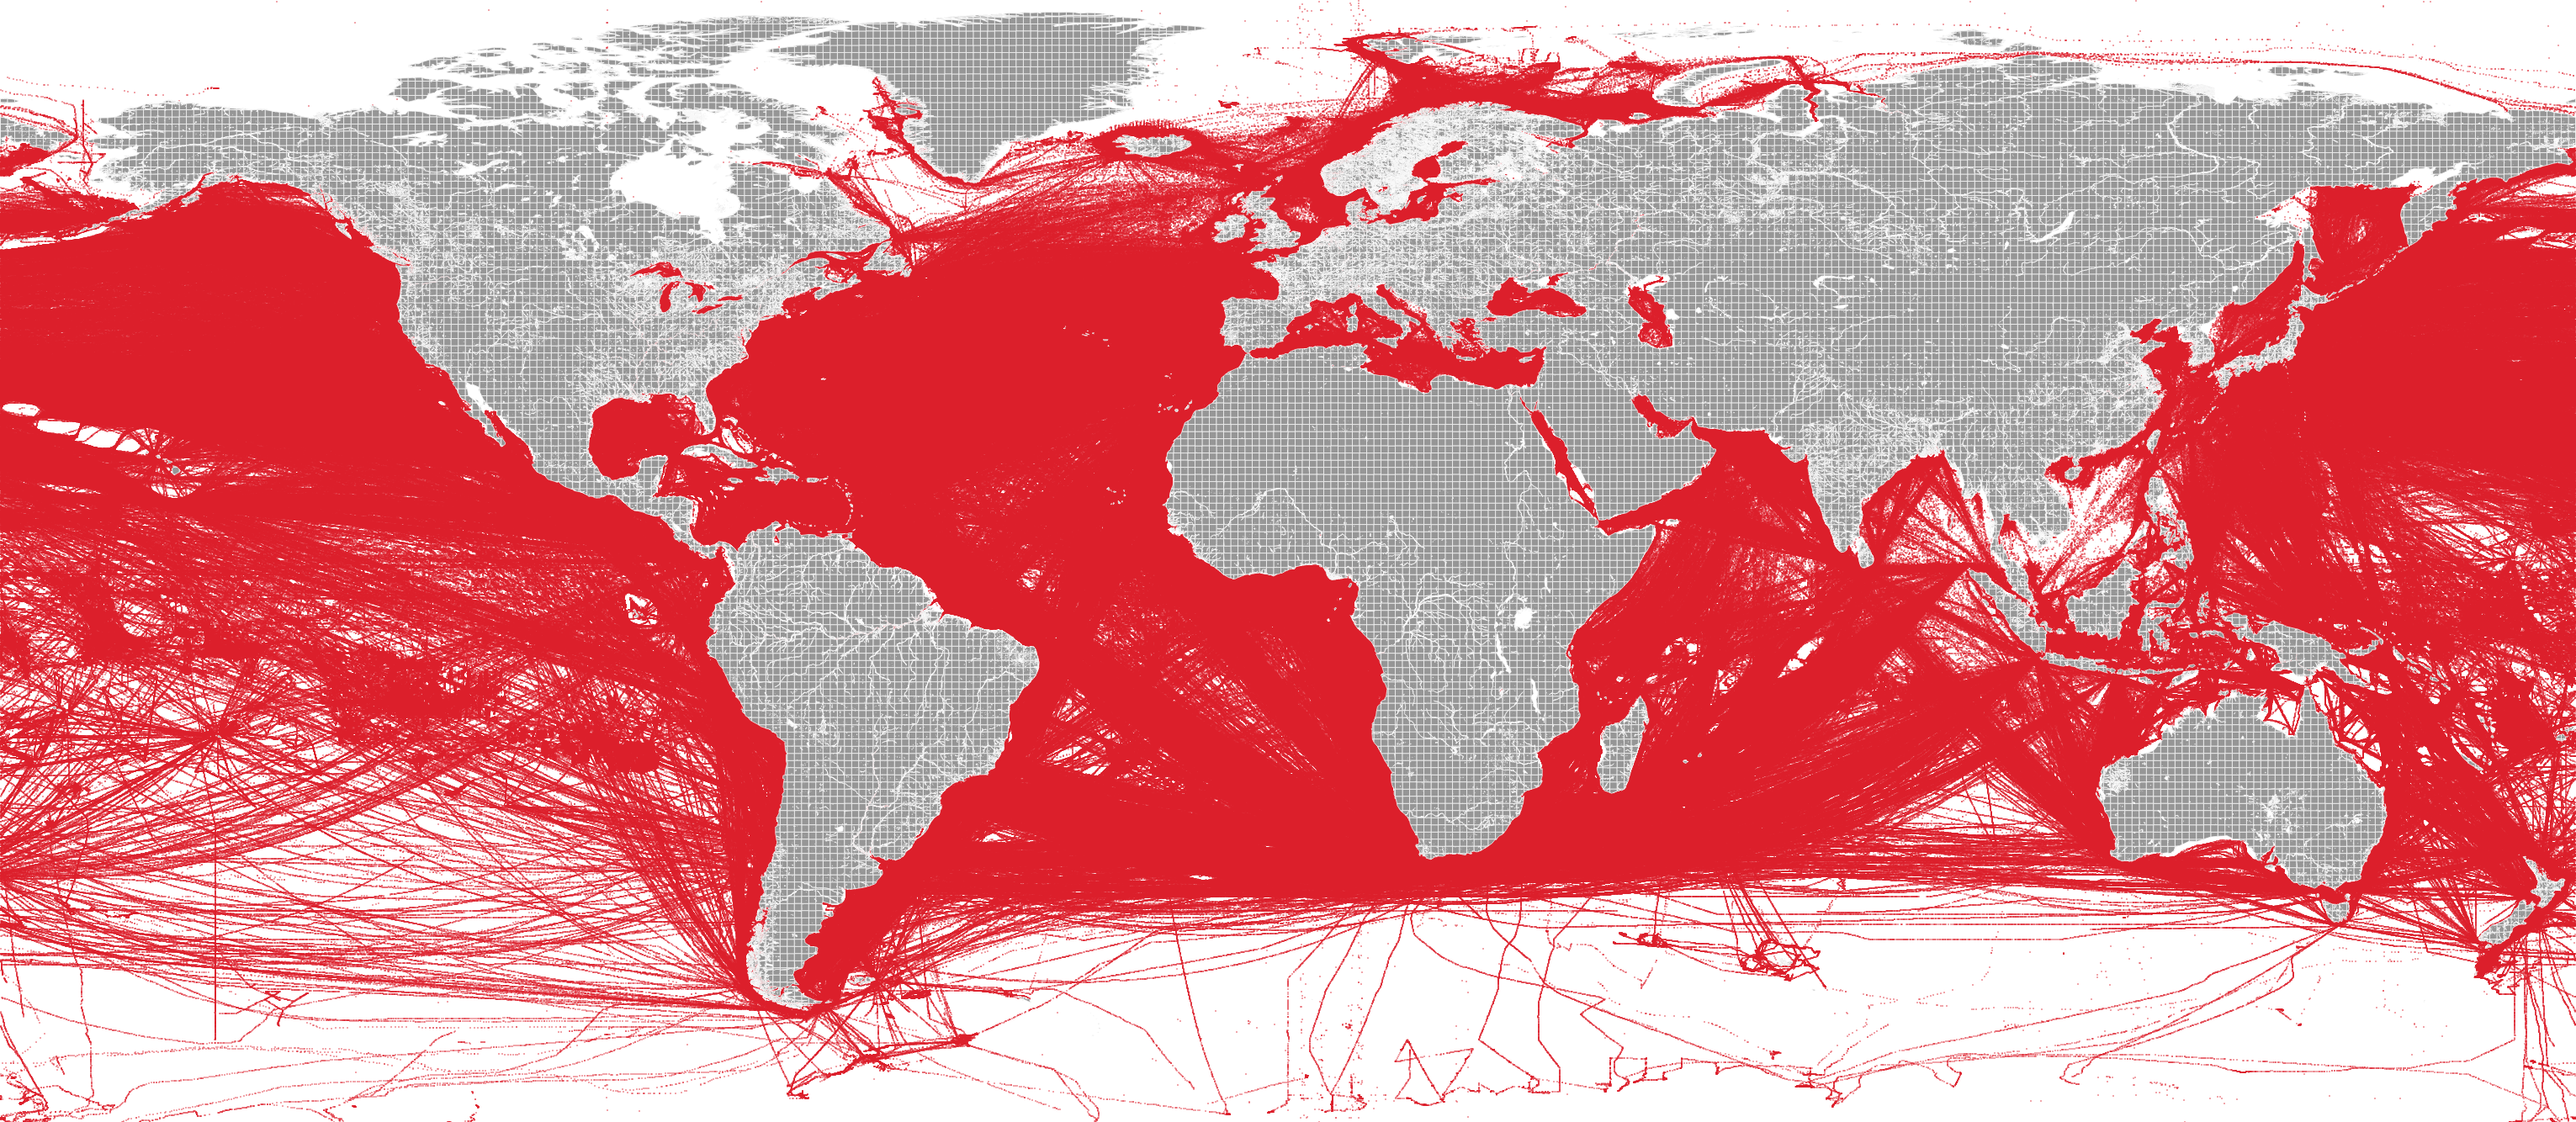
\includegraphics[width=1.0\textwidth]{figures/ais_positions}
    \caption{Vessel positions derived from 200 million AIS positional reports}
    \label{fig:ais_positions}
\end{figure}

As already mentioned in \cref{sec:topics_covered}, \acrfull{ais} was initiated by \acrfull{imo} and since 2004 every commercial and passenger vessel exceeding 299 \acrfull{gt} is required to carry an \acrshort{ais} transmitter. These transmitters broadcasts \acrshort{ais} messages following the \gls{aivdm} protocol. The \gls{aivdm} protocol contains two main types of reports: positional and static. The positional reports contains automatically collected information such as the transmitting vessel's \acrfull{mmsi} number, the current timestamp, and the vessel's current navigational data including the current geographical coordinates, \acrfull{sog}, \acrfull{cog}, true heading, \acrfull{rot}, and more. The static reports contain additional information about the vessel and its current voyage, some of which are manually inputted, such as the vessel's \acrshort{imo} number, name, dimensions, draft, intended destination and \acrfull{eta}. As an example, \cref{fig:ais_positions} shows a visualization of 200 million \acrshort{ais} randomly chosen positional reports from a collection of historical \acrshort{ais} positions for global collection of shipping vessels.

Regarding vessel identification there are mainly two values that are unique to a given vessel: the \acrshort{mmsi} and \acrshort{imo} numbers. Either of these should be unique on their own for a given vessel, however, \acrshort{mmsi} numbers can be recycled under certain conditions such as when a vessel is put out of commission while the \acrshort{imo} number is specific to a vessel's hull. Therefore, \acrshort{imo} is the preferred identifier, however, since the \gls{aivdm} protocol divides these identifiers in positional and static reports, both needs to be considered in order to use both static and positional \acrshort{ais} information.

\section{Additional vessel information and segmentation}

The collaborative company \acrfull{mo} has implemented a system for categorising vessels into different segments, subsegments, and further variations. This segmentations are based on various factors such as the dimensional data provided by \acrshort{ais} messages as well as details provided by external vessel information sources and even user and manual input. This segmentation of vessels is highly relevant to voyage patterns as vessels of different type and size travel to different ports and countries for different shipping companies. This is further shown in \cref{fig:segment_map} which shows, from an image of \acrshort{mo}'s web platform, how different subsegments of the dry bulk cargo segment travels in different areas of the world. Since this categorisation provides valuable insights into voyage patterns, vessel segmentation values are included in this thesis' proposed approach to vessel destination prediction.

\begin{figure}[htbp]  % order of priority: h here, t top, b bottom, p page
    \centering
    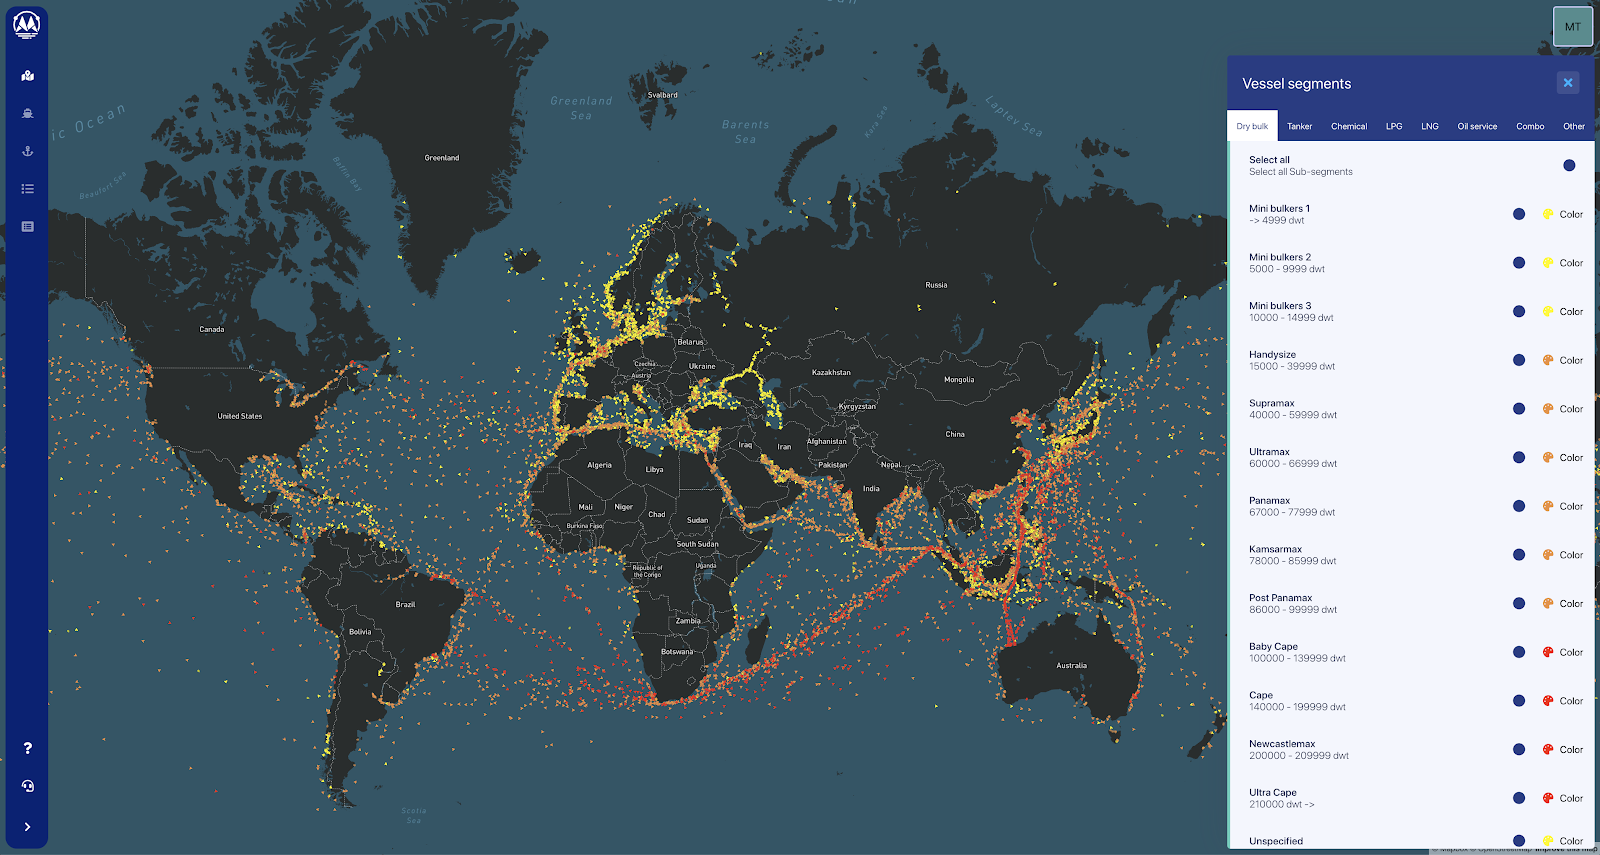
\includegraphics[width=1.0\textwidth]{figures/segment_map}
    \caption{\acrfull{mo}’s segmentation of vessels where yellow vessels are smaller than reds}
    \label{fig:segment_map}
\end{figure}


\section{Trajectory similarity}

As will be further elaborated on in \cref{chap:related_work}, the current literature related to vessel destination predictions almost exclusively rely on some form of trajectory similarity. Therefore, trajectory similarity is also included in this thesis' proposed approach to vessel destination prediction. There are three main categories of trajectory similarity measurements: spatial, temporal and tempo-spatial. Regarding vessel trajectories derived from \acrshort{ais}, they are not likely to share similar time intervals values as vessels travel at different speeds and at different times, therefore, for the purpose of this thesis, only spatial trajectory similarity measures are considered. This assumption is further corroborated by \cite{ZHANG2020102729} which arrived at a similar conclusion in their work to develop a \acrfull{ml} -based approach to trajectory similarity measurements.




\section{Machine learning (ML)}
